\chapter{Experimentos}

%El título del capítulo es flexible de acuerdo a cada tesis. Algunos títulos sugeridos podrían ser:
%\begin{itemize}
%\item El algoritmo X: nuestra propuesta.
%\item La técnica Y
%\end{itemize}
%Este título debe de estar ade acuerdo con el asesor del tema. Consúltelo en su sala de clase.

En este capítulo explicaremos la información necesaria y los procedimientos seguidos para llevar a cabo la experimentación. En primer lugar se explicarán los datasets que servirán de base y benchmark para los experimentos; luego se detallarán algunos detalles de la metodología; y finalmente se explicarán los experimentos a seguir.

\section{Datasets}

Los datasets que serán utilizados como casos de prueba son los siguientes:

\begin{description}
    \item[Apurata] Dataset privado de la fintech peruana con el mismo nombre
    \item[Lending Club] Dataset público de la mayor fintech de préstamo peer to peer en EE.UU.
    \item[Crédito Alemán] Dataset público de entidades bancarias Alemanas
\end{description}

Una mejor comparación entre estos datasets se puede encontrar en la tabla \ref{tab:dataset-comparison}

\begin{table}
    \centering
    \caption{Datasets utilizados}
    \label{tab:dataset-comparison}
    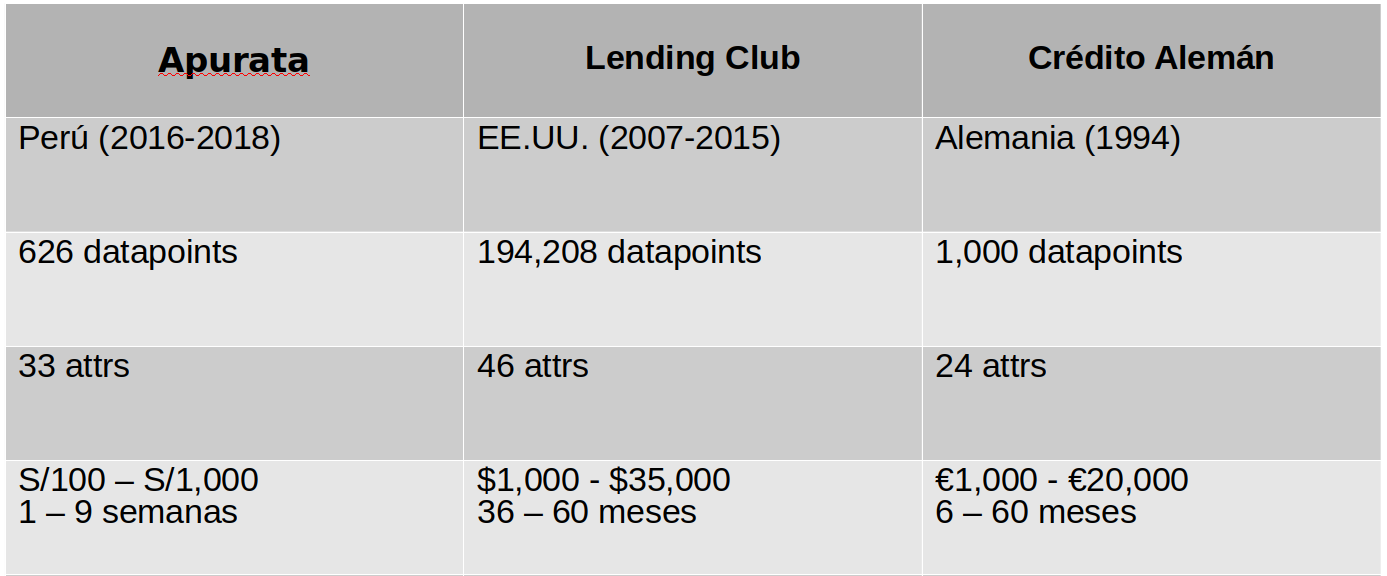
\includegraphics[width=0.8\linewidth]{graficos/dataset_comparison.png}
\end{table}

Como se puede apreciar, todos los datasets se componen de pocas variables, ninguno de ellos supera las 50. Los datasets de Apurata y del Crédito Alemán además son pequeños respecto a la cantidad de datapoints, con 1000 o menos registros.

También se cumple que los 3 conjuntos de datos son desbalanceados, ya que la clase de ``Default", o personas que no cumplieron con el pago de su deuda representa el 15\% para Apurata, 24\% para Lending Club y el 30\% para Crédito Alemán.

Por otro lado, los 3 datasets también poseen diferencias importantes entre sí que enriquecen su estudio. Apurata y Lending Club son fintech que utilizan diferentes criterios de los de los bancos para seleccionar su información. Los datasets de Crédito Alemán y Lending Club registran créditos que se realizan por montos más altos y a un mayor plazo que los de Apurata. Los periodos de tiempo y los países abarcados por los datasets también son únicos, y finalmente Lending Club tiene bastante más datapoints que los otros 2 datasets.

Los datasets de Crédito Alemán y Lending Club son considerados benchmark en sus respectivos sub-dominios, ya que hay varios estudios que los utilizan para realizar sus experimentos. Entre los que usan el dataset de Lending Club tenemos \cite{malekipirbazari2015risk, zhang2016research, zang2014credit, tan2018deep}. Y entre los que usan el dataset de Crédito Alemán tenemos \cite{harris2015credit, nanni2009experimental, brown2012experimental, wang2012two}.

\section{Metodología}

Para el preprocesamiento de la información, se eliminaron las variables con más del 50\% de información faltante, luego se eliminaron las filas con información faltante. A las variables resultantes se les convirtió a variables numéricas; y finalmente se hizo una normalización entre -1 y 1.

La interpretación de la variable $y$ se hizo de la siguiente manera: 1 para los buenos pagadores y 0 para los malos.

Para la selección de parámetros se realizó un grid-search con un ajuste fino manual al final. Sobre el desbalanceo de los datos, no se tomó ningún procedimiento especial. 

Para evaluar el desempeño de los modelos se hizo 10-fold validation 10 veces en Apurata y en el Crédito Alemán y 1 sola vez en Lending Club, ya que tiene abundante data. Finalmente se extrajo el promedio de todas las mediciones como la medición final. 

Las métricas utilizas son la accuracy, la precision, el recall y el AUC. La métrica que se buscó optimizar fue el AUC. Para las otras métricas se tuvo que seleccionar un punto de corte óptimo, que se escogió tratando de optimizar el accuracy, de modo que los resultados son comparables con el estado del arte.

\section{Experimentos}

En esta sección se describirán los experimentos llevados a cabo.

\subsection{Experimento 1}

El primer paso es hacer una comparación entre los clasificadores individuales y los ensambles de clasificadores (a partir de ahora lo abreviaremos como IB por imbalanced bagging). El objetivo de este experimento es verificar si efectivamente el desempeño mejora individualmente por cada clasificador, sin hacer una comparación transversal entre clasificadores de distintas familias.

En este experimento también evaluaremos la posibilidad de usar un algoritmo de aprendizaje profundo: \ac{DBN}.

\subsection{Experimento 2}

En este experimento compararemos los clasficadores IB con dos algoritmos de bagging usados ampliamente en la actualidad: \ac{RF} y \ac{XGBoost}. El objectivo de este experimento es verificar que el método de IB es competitivo con otros métodos de ensamble del estado del arte, sin el sesgo de haber usado una metodología diferente para el entrenamiento y la evaluación de los modelos.

\subsection{Experimento 3}

Finalmente en el experimento 3 compararemos los resultados obtenidos por nuestros clasificadores IB con los resultados obtenidos en otros estudios del estado del arte que usan los mismos datasets. El objetivo de este experimento es ratificar que los resultados son válidos para el estado del arte usando dos datasets benchmark.
